\documentclass[dvipsnames]{beamer}

\usepackage[utf8]{inputenc}
\usetheme{default}

\useinnertheme{circles}

%% set colours
\definecolor{atugreen}{HTML}{005b5e}
\setbeamercolor{title}{fg=atugreen}
\setbeamercolor{frametitle}{fg=atugreen}
\setbeamercolor{section in toc}{fg=atugreen}
\setbeamercolor{itemize item}{fg=atugreen}
\setbeamercolor{itemize subitem}{fg=orange}
\setbeamertemplate{section in toc}{\inserttocsectionnumber.~\inserttocsection}
\setbeamercolor{section number projected}{bg=white,fg=atugreen}

\title{Three data types:\\ continuous, coin flips and counts}
\author{Cóilín Minto, Olga Lyashevska}
\date{July 15\textsuperscript{th} 2022}
\institute{Marine and Freshwater Research Centre\\ Atlantic Technological University \\ Galway, Ireland}
%% logo
\titlegraphic{
    
\includegraphics[width=4cm]{figures/ATU-Logo-Full-RGB-Green-big.jpg}
}

\AtBeginSection[]{
\begin{frame}[noframenumbering, plain]
\frametitle{Outline}
\tableofcontents[currentsection]
\addtocounter{page}{-1}
\end{frame}
}

\begin{document}

\begin{frame}
 \maketitle
\end{frame}

\section{Data types}

%%------------------
%% CONTINUOUS DATA
%%------------------
\begin{frame}
 \frametitle{Describe some features of the response data $y$}
 \only<1>{
 \begin{center}
    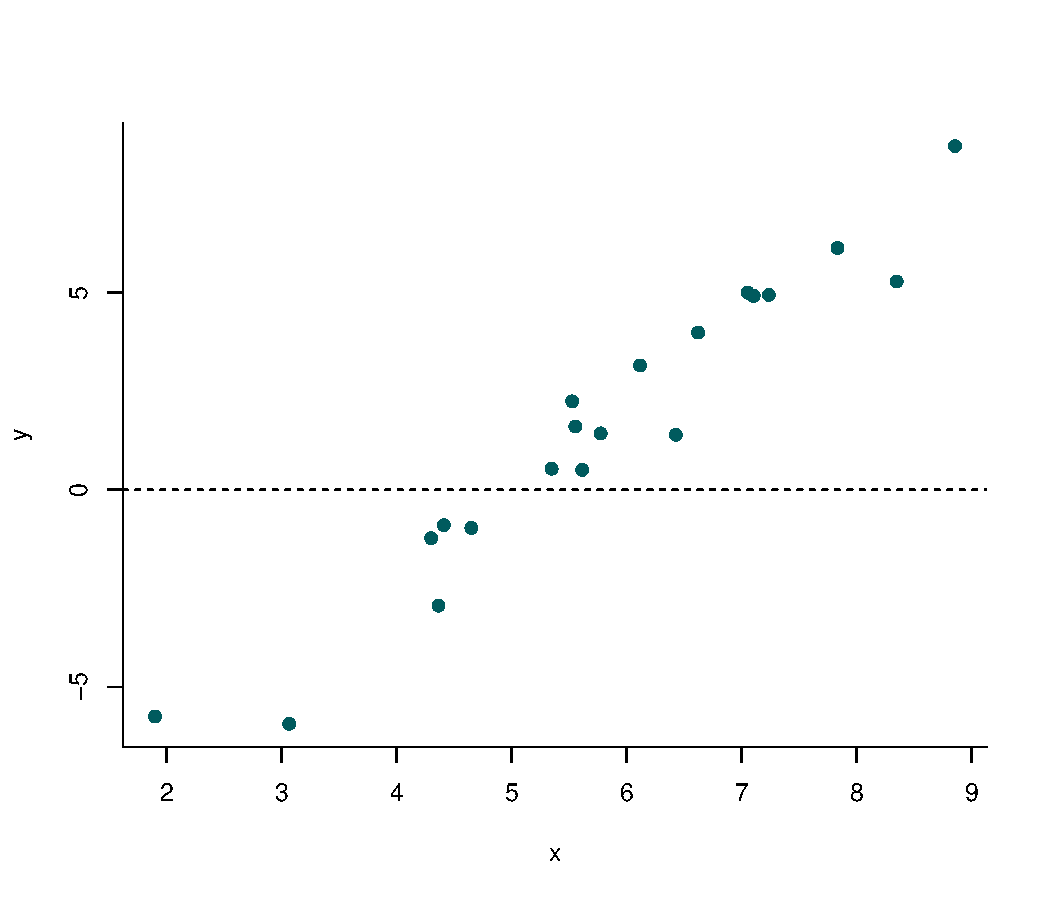
\includegraphics[width=10cm]{figures/continuous_y_0.pdf}
 \end{center}
} 
 \only<2>{
 \textcolor{atugreen}{{\bf Continuous data}}\vspace{.5cm}
 \begin{itemize}
  \item Response $y$ is continuous, e.g., $y = 1.25$ possible
  \item Response can be positive or negative (on the real line)
  \item Apparent positive linear relationship with continuous variable $x$
  \item {\bf Example} $y$ could be a change in water height
 \end{itemize}
} 
\end{frame}

%% positive continuous
\begin{frame}
 \frametitle{Describe some features of the response data $y$}
 \only<1>{
 \begin{center}
    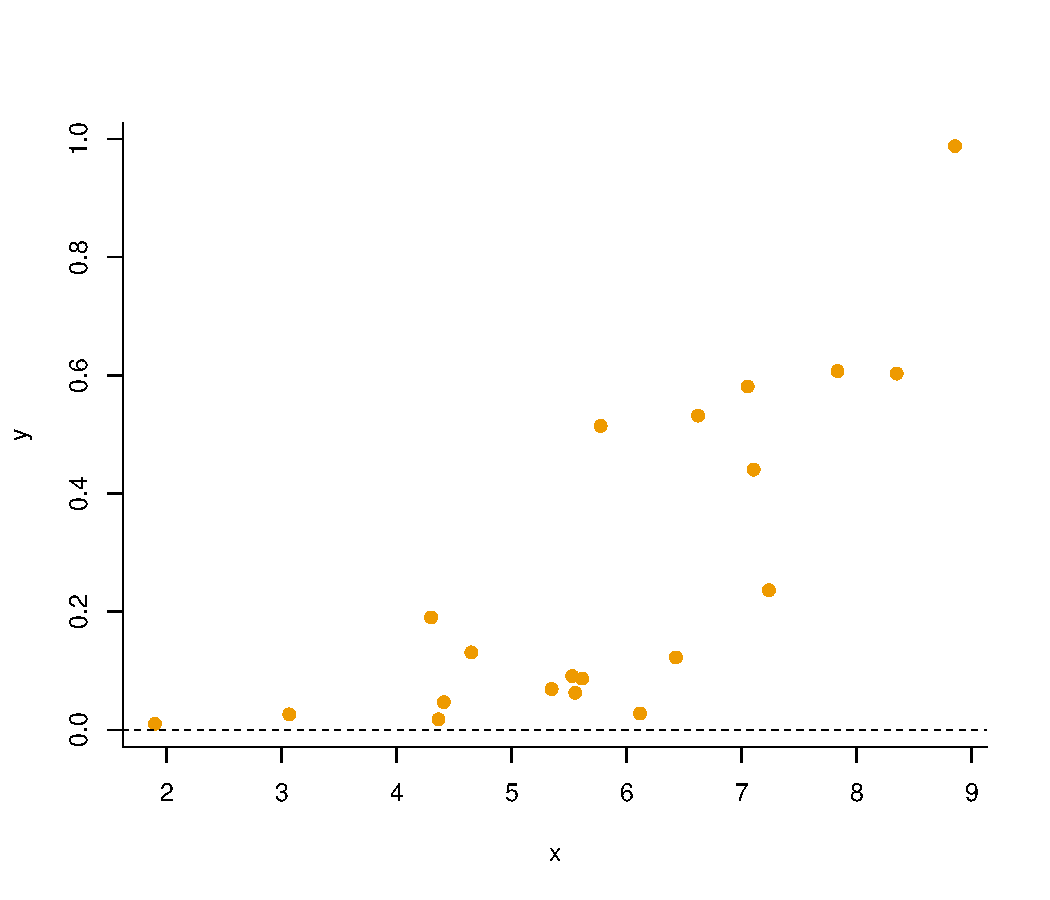
\includegraphics[width=10cm]{figures/continuous_y_1.pdf}
 \end{center}
} 
 \only<2>{
 \textcolor{Orange}{{\bf Positive continuous data}}\vspace{.5cm}  
 \begin{itemize}
  \item Response $y$ is also continuous, e.g., $y = 0.25$ possible
  \item Response can \underline{only} be positive (on the positive real line)
  \item Apparent positive non-linear relationship with continuous variable $x$
  \item {\bf Example} $y$ could be mass of individuals
   \begin{itemize}
    \item Discuss what values mass/weight of a fish could be
   \end{itemize}
 \end{itemize}
}
\end{frame}

%%------------------
%% COUNT DATA
%%------------------
\begin{frame}
 \frametitle{Describe some features of the response data $y$}
 \only<1>{
 \begin{center}
    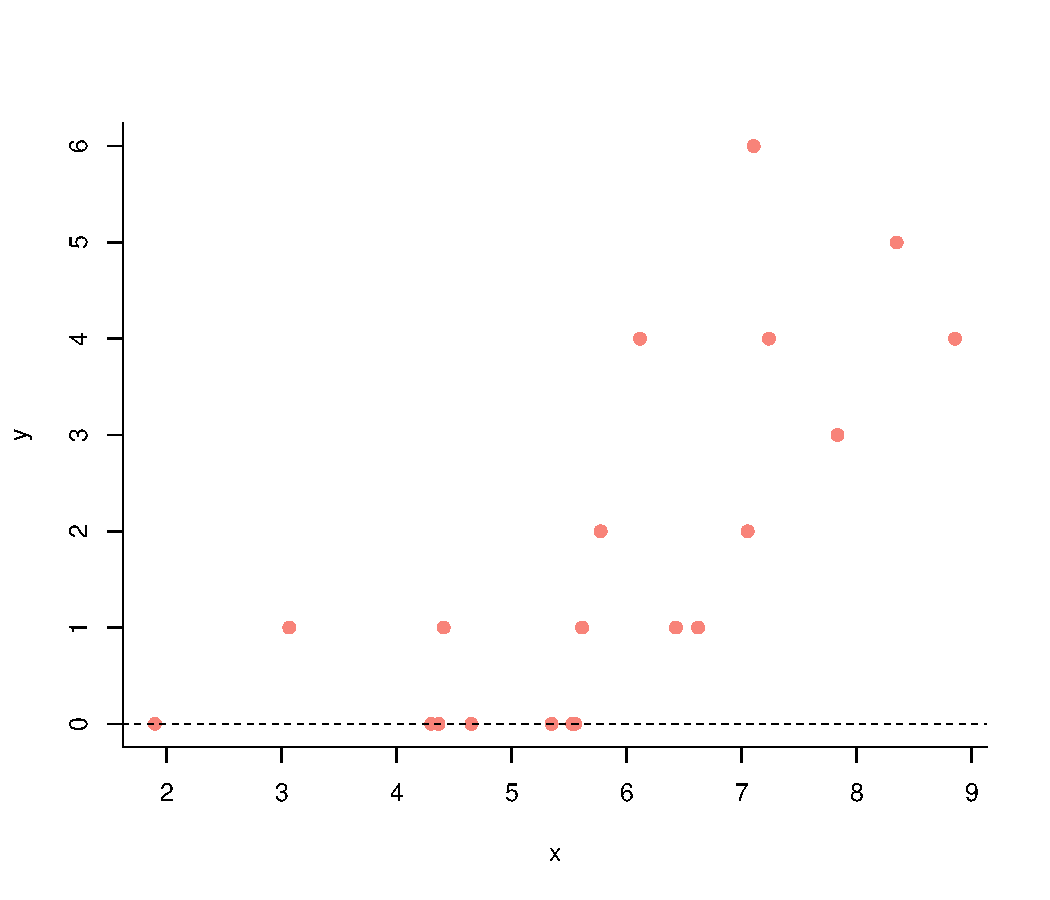
\includegraphics[width=10cm]{figures/count_y.pdf}
 \end{center}
} 
 \only<2>{
  \textcolor{Salmon}{{\bf Count data}}\vspace{.5cm}
 \begin{itemize}
  \item Response $y$ is a count (discrete), e.g., $y = 1.25$ impossible
  \item Response can be zero or a positive integer
  \item Apparent positive non-linear relationship with continuous variable $x$
  \item {\bf Example} $y$ could be abundance
   \begin{itemize}
    \item Discuss what values of abundance are possible
   \end{itemize}  
 \end{itemize}
} 
\end{frame}

%%------------------
%% BINARY DATA
%%------------------
\begin{frame}
 \frametitle{Describe some features of the response data $y$}
 \only<1>{
 \begin{center}
    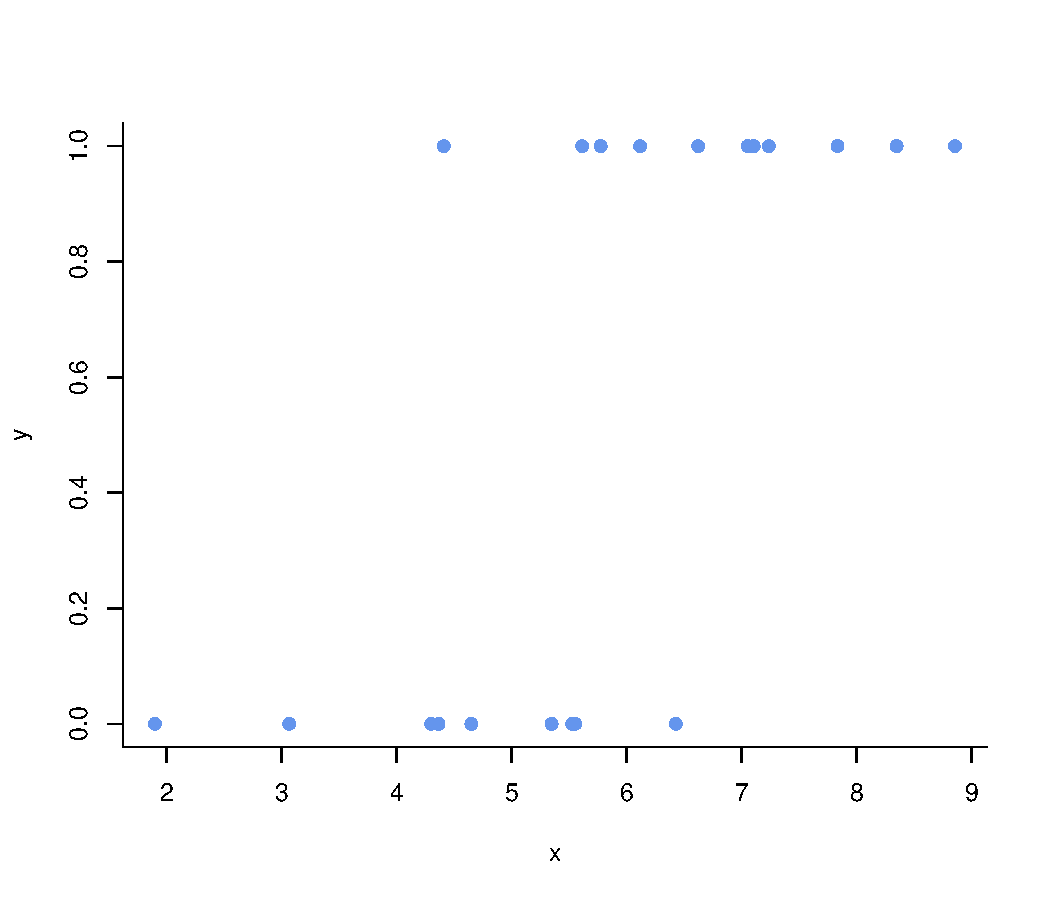
\includegraphics[width=10cm]{figures/binary_y.pdf}
 \end{center}
} 
 \only<2>{
  \textcolor{CornflowerBlue}{{\bf Binary data}}\vspace{.5cm}
 \begin{itemize}
  \item Response $y$ can be either a 1 or a 0 (or other binary categories) 
   \begin{itemize}
    \item Often it is a sum of positives out of a given number of trials, e.g., total number of heads in 10 coin flips
    \item Key thing is that for any one flip there can only be 2 outcomes
   \end{itemize}  
  \item Apparent positive non-linear relationship with continuous variable $x$
  \item {\bf Example} $y$ could be maturity status (mature/immature) for an organism
   \begin{itemize}
    \item Discuss other binary data examples
   \end{itemize}  
 \end{itemize}
} 
\end{frame}



\section{Probability distributions}

\begin{frame}
 \frametitle{Probability distribution}
 A function that describes the probabilities associated with possible outcomes for an experiment (think of the response $y$)
\end{frame}

\begin{frame}
 \frametitle{Continuous probability distributions}
 \only<1>{
% \vspace{-1cm}
 \begin{center}
  \textcolor{atugreen}{Normal distribution}
    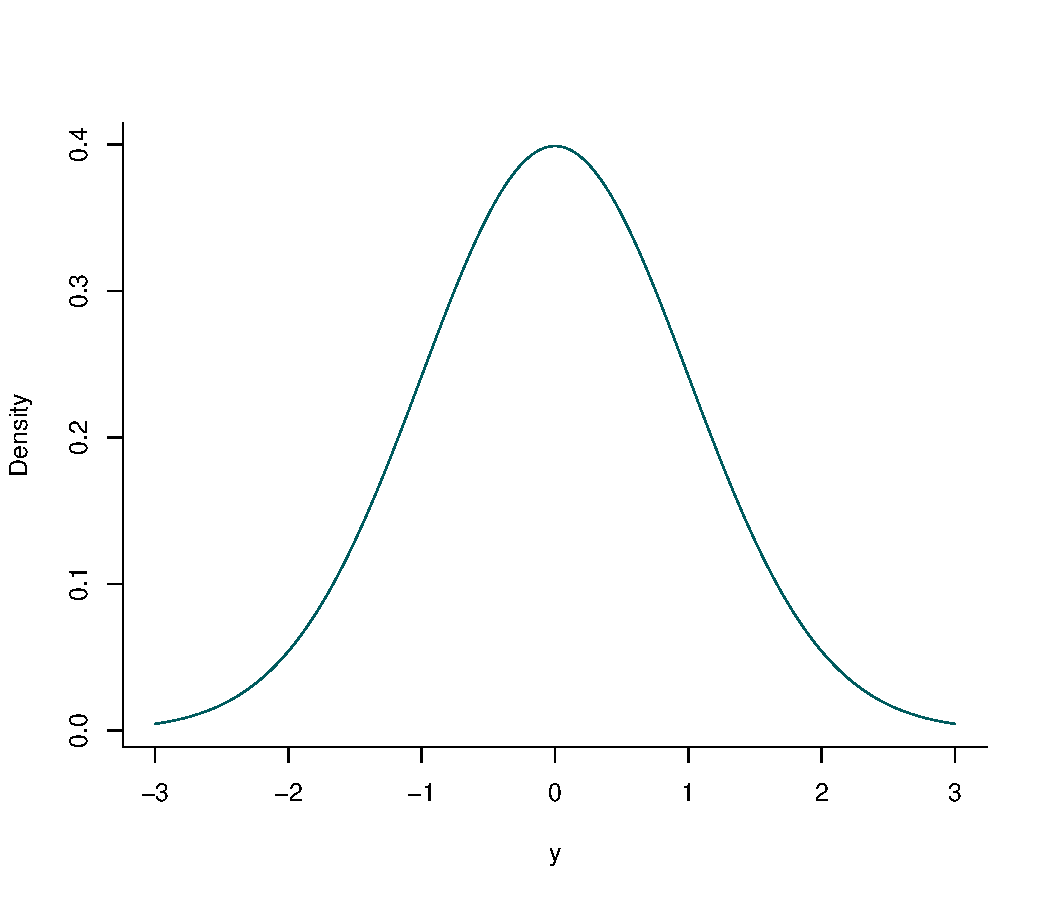
\includegraphics[width=9cm]{figures/normal_0.pdf}
 \end{center}
}
\end{frame}

\end{document}

\begin{frame}
 \frametitle{}
\end{frame}
